\documentclass[11pt]{article}
\usepackage{textcomp,bbding,subfig}
\usepackage{float,amssymb,amsmath,amsfonts,bm}
\usepackage{graphicx,cite}
\usepackage[]{natbib}
\def\style{apa}
\usepackage[usenames,pdftex,dvips]{color,xcolor}
\usepackage{multirow,tabulary,colortbl,array}
\usepackage[normalem]{ulem}
\usepackage[colorlinks,bookmarksopen,bookmarksnumbered,citecolor=blue,urlcolor=blue]{hyperref}
\usepackage{moreverb,setspace}

% Text layout
\topmargin -1.5cm
\oddsidemargin 0.0cm
\evensidemargin 0.0cm
\textwidth 16.5cm
\textheight 23.5cm
\setlength{\parindent}{0cm}

% Remove brackets from numbering in List of References
% \makeatletter \renewcommand\@biblabel[1]{} \makeatother
\makeatletter
\renewcommand{\@biblabel}[1]{\quad#1.}
\makeatother
% 
\allowdisplaybreaks[2]          % to accomodate long proofs spanning over pages
% 
% aliasis
\newcommand{\bs}{\boldsymbol}
\newcommand{\mean}[2]{\left\langle{#1}\right\rangle_{#2}}
\newcommand\numberthis{\addtocounter{equation}{1}\tag{\theequation}}
% 
% vectors and matrices
\newcommand{\vb}{\boldsymbol{b}}
\newcommand{\vc}{\boldsymbol{c}}
\newcommand{\vh}{\boldsymbol{h}}
\newcommand{\vv}{\boldsymbol{v}}
\newcommand{\vx}{\boldsymbol{x}}
\newcommand{\vw}{\boldsymbol{w}}
\newcommand{\vs}{\boldsymbol{s}}
% 
\newcommand{\md}{\boldsymbol{D}}
\newcommand{\mv}{\boldsymbol{V}}
\newcommand{\mh}{\boldsymbol{H}}
\newcommand{\mw}{\boldsymbol{W}}
\newcommand{\mx}{\boldsymbol{X}}
% 
% with hats or tildes
\newcommand{\vbt}{\tilde{\vb}}
\newcommand{\vct}{\tilde{\vc}}
\newcommand{\vht}{\tilde{\vh}}
\newcommand{\vvt}{\tilde{\vv}}
\newcommand{\vvp}{\vv^{\prime}}
\newcommand{\mwt}{\tilde{\mw}}
\newcommand{\vxt}{\tilde{\vx}}
\newcommand{\vhh}{\hat{\vh}}
\newcommand{\vvh}{\hat{\vv}}
% 
% xiaoran's edit
\newcommand{\xadd}[1]{\textcolor{blue}{#1}}
\newcommand{\xdel}[1]{\textcolor{red}{\sout{#1}}}
\newcommand{\xrpl}[2]{\xdel{#1}\xadd{#2}}
\newcommand{\xacc}[1]{\textcolor{ForestGreen}{#1}}
% 
% encoders
% vector or matrix
\newcommand{\vecEC}[1]{\boldsymbol{#1}}
% 
% decoders
\newcommand{\vecDC}[1]{\boldsymbol{\tilde{#1}}} 
% 
\newcommand{\xVO}{\boldsymbol{x}}         % the x vector, original
\newcommand{\xVR}{\boldsymbol{\tilde{x}}} % the x vector, recovered
\newcommand{\xSO}{x}                      % the x scaler, original
\newcommand{\xSR}{\tilde{x}}              % the x scaler, recovered
% 
% the vector of ones
\newcommand{\one}{\boldsymbol{1}}
% the diagnal matrix
\newcommand{\I}[1]{\boldsymbol{I}^{#1}}
% 
% parameters in the neural network
\newcommand{\Par}{\boldsymbol{\Theta}}
\newcommand{\pEC}{\boldsymbol{\theta}}
\newcommand{\pDC}{\boldsymbol{\tilde{\theta}}}
% 
% Loss function in Cross Entropy form
\newcommand{\LCE}[2]{#1\log{#2} + (1-#1)\log{(1-#2)}}
% 
% derivative
\newcommand{\DRV}[2]{\frac{d #1}{d #2}}
\newcommand{\DRC}[3]{\DRV{#1}{#2}\DRV{#2}{#3}}
\newcommand{\PDV}[2]{\frac{\partial #1}{\partial #2}}
\newcommand{\PDC}[3]{\PDV{#1}{#2}\PDV{#2}{#3}}
% 
% invers logit, aka. sigmoid function
\newcommand{\SGM}[1]{\frac{1}{1+e^{-#1}}}
% 
% assign to diagnoral
\newcommand{\diag}[1]{\text{diag} (#1)}
% 
% declarations
% argument of the minimum / maximum
\DeclareMathOperator*{\argmin}{arg\,min}
\DeclareMathOperator*{\argmax}{arg\,max}

% \pagestyle{headings}

% \author{Xiaoran Tong, Qin Lu} 
\doublespacing
\begin{document}
\title{An Joint Association Analysis Method for Genomic Sequencing and Neuroimaging Data}
\maketitle
\begin{flushleft}
  Xiaoran Tong\textsuperscript{1},
  Qin Lu\textsuperscript{1*},
  \\
  \bigskip
  \textbf{1} Department of Epidemiology and Biostatistics, Michigan State University, East Lansing, USA

  \vskip 50ex
  Correspondence: Qing Lu\\
  Department of Epidemiology and Biostatistics\\
  College of Human Medicine\\
  Michigan State University\\
  909 Fee Road\\
  East Lansing, MI 48824-1030\\
  qlu@msu.edu\\
\end{flushleft}

\clearpage
\begin{abstract}
  This research note covers the basics of Restricted Boltman Machine, a energy based, generative neural network.
\end{abstract}
\clearpage

\section{Boltzmann Machine}
\subsection{Concept}
A Boltzmann Machine (BM) is an engergy based model for binary data generation process, who views the observed data as the fraction of a physics system on display. In the complete system, the observed $P$ dimensional data is in fact the realization of its $P$ visible units, denoted by vector $\vv$, besides which there are presumably $Q$ hidden units holding unobserved data, denoted by vector $\vh$. All units are allowed to connect with each other to form mutual dependencies, as Figure \ref{fig:gbm} illustrates.
\begin{figure}[h]
  \centering
  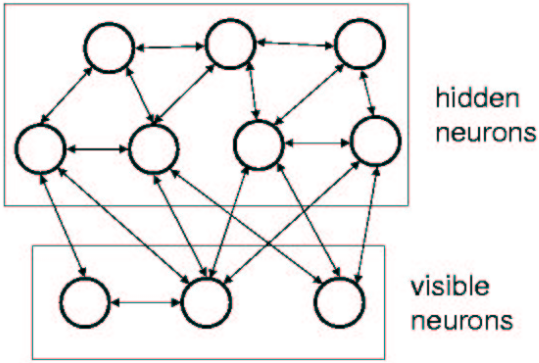
\includegraphics[width=200px]{img/gbm.png}
  \caption{General Boltzmann Machine.}\label{fig:gbm}
\end{figure} \\
Together, the assignment of $\vv$ and $\vh$ comprices a complete $P+Q$ dimensional state vector $\vs =(\vv, \vh)$ of the system. Each distinct state is characterized by its energy, measurable by an energy function $E(\vs) = E(\vv, \vh)$. By the rule of nature, when a system reaches thermal equilibrium, states of lower engery are more likelly to sustain (thus more prevalent) than those of higher energy. Upholding this rule, the probability of a specific state $\vs=(\vv, \vh)$ presenting itself in the system, is proportional to the exponential of the negative energy of the said state, that is,
\begin{equation} \label{eq:p(s)}  % probability of observing a complete state
  \begin{split}
    \Pr(\vs) = \Pr(\vv, \vh) = \frac{e^{-E(\vv, \vh)}}{Z}, \quad Z = \int_{\vv,\vh} e^{-E(\vv, \vh) \,d\vv\,d\vh},
  \end{split}
\end{equation}
which is a Boltzmann distribution that assigns lower engery states higher density and vise versa. The partition function $Z$ serves as a normalizing constant to ensure $\int_{\vv, \vh} \Pr(\vv, \vh) \,d\vv\,d\vh = 1$. It is readily seen that engergy function $E(\vv, \vh)$ determines the system's dynamic behovior, it is therefore carefully choosen to allow emulation of the natural process that have given rise to the binary visible data we have collected. A Boltzmann Machine defines a binary system with energy function
\begin{align*}\label{eq:e(s)} % system energy for generic boltzmann machine
    E(\vv, \vh) = E(\vs) = -\sum_{i=1}^{P+Q} b_i s_i - \sum_{1 = i < j}^{P+Q} s_i w_{ij} s_j \numberthis
\end{align*}
where $b_i$ is an offest, serving as the thresholds for the $i$ th unit to switch from ``off'' to ``on'' state; $w_ij$ is the connection between the $i$ th and $j$ th units. The first term depicts that an total energy no less than an unit's threshold is required to maintain that unit's ``on'' state; the second terms says that extra energy is required to sustain a active mutual connection when the two units at both ends are ``on''. The energy function is thus paramterized by $P+Q$ offsets and $P+Q \choose 2$ undirected connections, we represent them by $\pEC = \{b_i, m_{ij} | 1 \le i < j \le P+Q\}$. \\
A1: The probability of a particular unit $s_k, (k = 1, \dots, P+Q)$ being turned on is
\begin{equation}\label{eq:p(s_k=1)}
  \Pr(s_k = 1) = \sigma(b_k + \sum_{i=1, i \ne k}^{P+Q}{s_i w_{ik}})
\end{equation}
Here,  $\sigma(x) = [1 + \exp({-x})]^{-1}$ is the sigmoid (logistic) function. \\
Proof: start by splitting the energy contributed by the $k$ th unit from the rest,
\newcommand{\st}{\tilde{s}}
\begin{align*}
  E(\vs)
  & = \left( -\sum_{i=1, i \ne k}^{P+Q} b_i s_i - \sum_{1 \le i < j, i \ne k, j \ne k}^{P+Q} s_i w_{ij} s_j \right) + \left(-b_k s_k - \sum_{i=1, i \ne k}^{P+Q}s_i w_{ik} s_k \right) \\
  & = E(\vs_{-k}) + E(s_k), \\
  \Rightarrow \Pr(s_k)
  & = \int_{\vs_{-k}} \Pr(\vs) d\vs_{-k} = \frac{1}{Z} \int_{\vs_{-k}} e^{-E(\vs)} d\vs_{-k} \Leftarrow (\ref{eq:p(s)}) \\
  & = \frac{\int_{\vs_{-k}} e^{-E(\vs)} d\vs_{-k}}{\int_{\vs} e^{-E(\vs)} d\vs} \\
  & = \frac{e^{-E(s_k)} \int_{\vs_{-k}} e^{-E(\vs_{-k})} d\vs_{-k}}  {\int_{\st_k} \int_{\vs_{-k}} e^{-E(\vs_{-k})} d\vs_{-k}\,d\st_k} \\
  & = \frac{e^{-E(s_k)} \int_{\vs_{-k}} e^{-E(\vs_{-k})} d\vs_{-k}}  {[e^{-E(\st_k)}|_{\st_k=1} + e^{-E(\st_k)}|_{\st_k=0}] \int_{\vs_{-k}} e^{-E(\vs_{-k})} d\vs_{-k}} \\
  & = \frac{e^{-E(s_k)}}{e^{-E(\st_k)}|_{\st_k=1} + e^{-E(\st_k)}|_{\st_k=0}} \\
  % 
  \Rightarrow \Pr(s_k=1)
  & = \frac{e^{-E(s_k)}|_{s_k=1}}{e^{-E(\st_k)}|_{\st_k=1} + e^{-E(\st_k)}|_{\st_k=0}} \\
  & = \frac{e^{b_k + \sum_{i=1, i \ne k}^{P+Q}{s_i w_{ik}}}}{e^{b_k + \sum_{i=1, i \ne k}^{P+Q}{s_i w_{ik}}} + e^{0}} \\
  & = \frac{1}{1 + e^{-b_k - \sum_{i=1, i \ne k}^{P+Q}{s_i w_{ik}}}} \\
  & = \sigma(b_k + \sum_{i=1, i \ne k}^{P+Q}{s_i w_{ik}})
\end{align*}
\subsection{MLE for Boltzmann Machine}
The best interest is to fine tune the flexible parameters $\pEC=\{b_i, w_{ij} | 1 \le i < j \le P+Q \}$ in such a way that the odds of observing the $N$ empirical data points $\mv=[\vv_1, \dots, \vv_N]^T$ on the visible units are maximized, which is equivalent to maximizing the marginal Boltzman distribution $\Pr(\vv, \vh)$ over assignments of $\vh$:
\begin{equation} \label{eq:p(v)}  % probability of observing a visible portion
  \begin{split}
    \Pr(\vv) = \int_{\vh}{\Pr(\vv, \vh)d\vh} = \frac{1}{Z} \int_{\vh}{e^{-E(\vv, \vh)}d\vh}.
  \end{split}
\end{equation}
The tuning requires the gradient of negative log likelihood with respect to $\pEC$ to decide updating rules, such that
\[ \pEC^{t+1} = \pEC^t + \epsilon \PDV{-\log{\Pr(\vv)}}{\pEC}, \]
where $\pEC^{t+1}$ is the resulting parameters of $t$ iterative updates, and $\epsilon$ is the learning rate. Now introduce the gradient expression:
\begin{align}\label{eq:gv1}
  -\PDV{\log{\Pr(\vv)}}{\pEC} &= -\PDV{\log{\int_{\vh}{e^{-E(\vv, \vh)}d\vh}}}{\pEC} + \PDV{\mean{\log{\int_{\vh}{e^{-E(\vvt, \vh)}d\vh}}}{\vvt}}{\pEC}.
\end{align}
The angled bracket $\mean{\dots}{\mx}$ denotes the expected value of an expression over random variable $\mx$.
There are a number of ways to interpret the gradient terms. The first term (without sign) is referred as \textbf{positive phase}, due to the fact that increases this term increases the likelihood of $\vv$; for the same reason, the second term (without sign) is called \textbf{negative phase}.\\
Derivation of (\ref{eq:gv1}):
\begin{align*}
  -\PDV{\log{\Pr(\vv)}}{\pEC}
  & = -\PDV{\log{\int_{\vh}{e^{-E(\vv, \vh)}d\vh}}}{\pEC} + \PDV{\log{\int_{\vvt, \vh} e^{-E(\vvt, \vh)} d\vvt\,d\vh }}{\pEC} \quad \Leftarrow (\ref{eq:p(s)}, \ref{eq:p(v)}) \\
  \textrm{\textbf{Positive phase:}} & \textrm{ Done!} \\
  \textrm{\textbf{Negative phase:}} \\
  \PDV{\log{\int_{\vvt, \vh} e^{-E(\vvt, \vh)} d\vvt\,d\vh }}{\pEC}
  & = \frac{1}{\int_{\vvt, \vh} e^{-E(\vvt, \vh)} d\vvt\,d\vh} \PDV{\int_{\vvt}\int_{\vh} e^{-E(\vvt, \vh)} d\vh\,d\vvt}{\pEC} \\
  & = \frac{1}{Z} \int_{\vvt} \PDV{ \int_{\vh}{e^{-E(\vvt, \vh)}}d\vh }{ \pEC } d\vvt \quad \Leftarrow (\ref{eq:p(s)}),\,\textrm{sum rule in deferenciation} \\
  & = \int_{\vvt}  \frac{1}{Z}\int_{\vh} e^{-E(\vvt, \vh)} d\vh \PDV{\log{\int_{\vh} e^{-E(\vvt, \vh) d\vh}}}{\pEC}  d\vvt \quad \Leftarrow \PDV{f(\vx)}{\vx}=f(\vx)\PDV{\log{f(\vx)}}{\vx} \\
  & = \int_{\vvt}{\Pr(\vvt) \PDV{\log{\int_{\vh}{e^{-E(\vvt, \vh)}d\vh}}}{\pEC}}d\vvt \quad \Leftarrow (\ref{eq:p(v)}) \\
  & = \mean{\PDV{\log{\int_{\vh}{e^{-E(\vvt, \vh)}d\vh}}}{\pEC}}{\vvt} \\
  & = \PDV{\mean{\log{\int_{\vh}{e^{-E(\vvt, \vh)}d\vh}}}{\vvt}}{\pEC} \quad (\textrm{Done!}).
\end{align*}
The above gradient form (\ref{eq:gv1}) is not ideal for direct implementation, since the update rule still involves gradient for both positive and negative phase, but it is meant for symbolic expression packages such as python theano which automatically program gradient function once the objective (or pseudo objective) function has been programmed. For low level implementation though, the update rules has to be gradient free, rearrange (\ref{eq:gv1}) we see
\begin{align*}
  \textrm{Positive Phase:}
  & \\
  \PDV{\log{\int_{\vh}{e^{-E(\vv, \vh)}d\vh}}}{\pEC} 
  & = \frac{1}{\int_{\vht} e^{-E(\vv, \vht)} d\vht}   \PDV{\int_{\vh} e^{-E(\vv, \vh)} d\vh}{\pEC}  \\
  & = \frac{1}{\int_{\vht} e^{-E(\vv, \vht)} d\vht}   \int_{\vh} \PDV{ e^{-E(\vv, \vh)}}{\pEC} d\vh \\
  & = \frac{1}{\int_{\vht} e^{-E(\vv, \vht)} d\vht}   \int_{\vh} e^{-E(\vv, \vh)}\PDV{-E(\vv, \vh)}{\pEC} d\vh \\
  & = \frac{1}{ \frac{1}{Z}  \int_{\vht} e^{-E(\vv, \vht)} d\vht}  \int_{\vh} \frac{e^{-E(\vv, \vh)}}{Z} \PDV{-E(\vv, \vh)}{\pEC} d\vh \\
  & = \frac{1}{\Pr(\vv)}  \int_{\vh} \Pr(\vv, \vh)\PDV{-E(\vv, \vh)}{\pEC} d\vh  & \Leftarrow (\ref{eq:p(s)})(\ref{eq:p(v)}) \\
  & = -\int_{\vh} \frac{\Pr(\vv, \vh)}{\Pr(\vv)} \PDV{E(\vv, \vh)}{\pEC} d\vh \\
  & = -\int_{\vh} \Pr(\vh | \vv) \PDV{E(\vv, \vh)}{\pEC}  d\vh \\
  & = -\mean{\PDV{E(\vv, \vh)}{\pEC}}{\vh|\vv} \\
  \textrm{Negative Phase:}
  & \\
  \PDV{\mean{\log{\int_{\vht}{e^{-E(\vvt, \vht)}d\vht}}}{\vvt}}{\pEC}
  &= \mean{\PDV{\log{\int_{\vht}{e^{-E(\vvt, \vht)}d\vht}}}{\pEC}}{\vvt} \\
  &= \mean{ -\mean{\PDV{E(\vvt, \vht)}{\pEC}}{\vht|\vvt}  }{\vvt} \\
  &= -\mean{\PDV{E(\vvt, \vht)}{\pEC}}{\vvt, \vht}.
\end{align*} 
Thus we could rewrite ({\ref{eq:gv1}) in terms of expected value:
\begin{align} \label{eq:gv2}
  -\PDV{\log{\Pr(\vv)}}{\pEC} = \mean{\PDV{E(\vv, \vh)}{\pEC}}{\vh|\vv} - \mean{\PDV{E(\vvt, \vht)}{\pEC}}{\vvt, \vht}
\end{align}
The gradients still exists on the right side, but it only involves energy function itself without either logarithm or exponentiation. The earlier positive and negative phases (see \ref{eq:gv1}) are now re-expressed by two expectation terms, which is commonly referred as \textbf{data} phase and \textbf{model} phase, because the former are influenced by actual data $\vv$ from observation through conditioning , and is contributing to its chance of being generated by the Boltzmann Machine; while the later is based on the Boltzmann Machine (the model) entirely, without any substantial data from observation, which contributes to the likelihood of the ``full data'' including those presented on the hidden units, but also relatively diminishes the marginal likelihood of empirical data $\vv$ on the visible units. \\
Another way to interprete (\ref{eq:gv2}) is to view the ``loss'' being the difference of mean energy between a system runing with $P$ visible units hard wired to empirical observation $\vv$, and the same system freely run without the said constraint; thus minimizing this ``loss'' via negative gradient amounts to urge the machine to put $\vvt$ on its visible units, which mimics the reality $\vv$ as closely as possible. \\
Now, taking advantage of the simple form of energy function for a Boltzmann distribution (equation \ref{eq:e(s)}), we immediately see
\begin{align} \label{eq:ge}
  \PDV{E(\vs)}{w_{ij}} = s_i s_j,  \quad \PDV{E(\vs)}{b_i} = s_i, \quad  (1 \le i < j \le P+Q)
\end{align}
Joint (\ref{eq:ge}) and (\ref{eq:gv2}) we get the primative update rules for the MLE of $\Pr(\vv)$:
\begin{align*} \label{eq:gv3}
  -\PDV{\log{\Pr(\vv)}}{w_{ij}} &= \mean{s_i s_j}{\vh|\vv} - \mean{s_i s_j}{\vvt, \vht} \\
  -\PDV{\log{\Pr(\vv)}}{b_i}    &= \mean{s_i}{\vh|\vv} - \mean{s_i}{\vvt, \vht} \numberthis \\
  \textrm{where }               & 1 \le i < j \le P+Q.
\end{align*}
The interpretation of update rules are quiet straight forward, for $w_{ij}$, the connection between $s_i$ and $s_j$, it is the difference of unit $i$ and $j$'s covariance between a system clumped on visible units and the same system that has been set free; as for $b_i$, the unit offset (activation threshold) of $s_i$, the update is the difference of mean value on the $i$ th unit, between a clumped and free run systems. At this point, we are readly to train a Bolztmann Machine by iteration:
\begin{itemize}
\item \textbf{Positive/Data} Phase:
  \begin{itemize}
  \item clump the observed $P$ dimensional sample onto the $P$ visible units $\vv$;
  \item simulate the ``thermal'' dynamics of $Q$ hidden units according to (\ref{eq:p(s_k=1)});
  \item repeat until the values on $\vh$ reaches ``thermal'' equilibrium (burn in);
  \item repeat some more time (sampling), \\
    estimate $\mean{s_i s_j}{\vh|\vv}$ by the proportion of times both unit $i$ and $j$ are on; \\
    estimate $\mean{s_i}{\vh|\vv}$ by the proportion of times unit $i$ is on;
  \end{itemize}
\item \textbf{Negative/Model} Phase:
  \begin{itemize}
  \item relax the constraint on the $P$ visible units;
  \item simulate the ``thermal'' dynamics of all $P + Q$ units according to (\ref{eq:p(s_k=1)});
  \item repeat until the values on $(\vv, \vh)$ reaches ``thermal'' equilibrium (burn in);
  \item repeat some more time (sampling), \\
    estimate $\mean{s_i s_j}{\vv, \vh}$ by the proportion of times both unit $i$ and $j$ are on; \\
    estimate $\mean{s_i}{\vv, \vh}$ by the proportion of times unit $i$ is on;
  \end{itemize}
\item Update:
  \begin{itemize}
  \item \quad $w_{ij}^{(t+1)} = w_{ij}^{(t)} + \epsilon (\mean{s_i s_j}{\vh|\vv} - \mean{s_i s_j}{\vv, \vh})$
  \item \quad $b_i^{(t+1)}    = b_i^{(t)}    + \epsilon (\mean{s_i    }{\vh|\vv} - \mean{s_i    }{\vv, \vh})$
  \end{itemize}
\item Repeat until all $w_{ij}$ and $b_i$ converges.
\end{itemize}
% new subsection
\subsection{MLE with Symbolic Library}
The primative update rules is necessary for developing a BM trainer from scratch, but in case of available symbolic mathematics libraries such as Python-Theano and Matlab-Symbolics, it is often unnecessary or even over-developing to implement the primative rules in equ \ref{eq:gv3}. Instead, it would be more efficient and easier to just specify the objective (or even puesdo objective) function (\ref{eq:gv1}), and let the software packages to figure out the gradient function, and subsequently, the update rules.
Review the negative log likelihood gradient in equation \ref{eq:gv1}, we see the objective function to be minimized with respect to $\pEC$, is actually
\begin{align}\label{eq:l(v)1}
  L(\vv; \pEC) = -\log{\int_{\vh}{e^{-E(\vv, \vh)}d\vh}} + \mean{\log{\int_{\vh}{e^{-E(\vvt, \vh)}d\vh}}}{\vvt}
\end{align}
which involves the mean of marginal distribution $\Pr(\vvt)$, posing a severe challenge to direct evaluation attempt, we instead resort to approximation via limited sampling from $\Pr(\vvt)$:
\begin{align}\label{eq:l(v)2}
  L(\vv; \pEC) \approx -\log{\int_{\vh} e^{-E(\vv, \vh)} d\vh} + \frac{1}{|M|}\sum_{\vvt \in M}{\log{\int_{\vh} e^{-E(\vvt, \vh)}d\vh}}
\end{align}
where $M$ is the set of samples drawn from $\Pr(\vvt)$. \\
It is now helpfult to introduce the notion of ``free energy'' $F$, which, just likes the complete energy $E$ that corresponds to each distinct state $\vs=(\vv, \vh)$, corresponds to every distinct visible state $\vv$. Free energy takes the form:
\begin{equation}\label{eq:f(v)}
  \begin{split}
    F(\vv) &= -\log{\int_{\vh}{e^{-E(\vv, \vh)}d\vh}}.
  \end{split}
\end{equation}
Compare (\ref{eq:f(v)}) with (\ref{eq:e(s)}), we see that $F(\vv)$ is actually the kernel of $\Pr(\vv)$ which is the marginal distribution of $Pr(\vv, \vh)$ over $\vh$ under the negative log scale. Refer to (\ref{eq:p(s)}), $F(\vv)$ governs the system in the same manner, allbeit the only concern of $F(\vv)$ is the visible portion:
\begin{align}\label{eq:p(v)|fe}
    \Pr(\vv) = \frac{e^{-F(\vv)}}{Z}, \quad\quad Z=\int_{\vv}{e^{-F(\vv)}}d\vv
\end{align}
It makes the aforementioned gradient expression more concise:
\begin{align}\label{eq:grad3}
  -\PDV{\log{\Pr(\vv)}}{\pEC} \approx \PDV{F(\vv)}{\pEC} - \PDV{\frac{1}{|M|}\sum_{\vvt \in M}{F(\vvt)}}{\pEC},
\end{align}
\subsection{Theano Implementation}
For Python-Theano users, is would be best to utilize Theano's symbolic gradiant solver. From the gradient form in either (\ref{eq:gv2}) or (\ref{eq:gv3}), we could consider the numerator portion as the objective funtion $L(\vv; \pEC)$ to be minimized by stochastic gradient descent (SGD)[?], such that,
\begin{align}
  L(\vv) = F(\vv) - \frac{1}{|M|}\sum_{\vvt \in M}{F(\vvt)},
\end{align}
where $F(\vv)$ depends on $E(\vv, \vh)$ which is further parameterized by $\pEC$; $\vv$, $\vh$ and the limited samples $\vvt \in M$ are all considered constant, and we will let Theano to figure out the gradient function $\PDV{L(\vv)}{\pEC}$

\section{Binary RBM}
In a generic Bolzmann Machine (GBM), all units are allowed to connect with each other, the preceding adjective ``Restricted'' highlights an additional constraint that connection is forbidden among visible units themselves, and among hidden units as well, only those between the two group are allowed, as Figure \ref{fig:rbm} illustrates.
\begin{figure}[h]
  \centering
  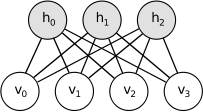
\includegraphics[width=100px]{img/rbm.png}
  \caption{The Restricted Boltzmann Machine.}\label{fig:rbm}
\end{figure}
The behavior of the system is determined by the engergy function $E(\vv, \vh)$, parameterized by $\pEC$. We now limit the discussion on the most heavily researched binary systems, that is, the entries in $\vv$ and $\vh$ are only taken from $\{0, 1\}$. The energy $E(\vv, \vh)$ is formulated by:
\begin{equation} \label{eq:se_bin}
  E(\vv, \vh) = -\vb^T \vv - \vc^T \vh - \vh^T \mw \vv,
\end{equation}
where the entries in the P-dimensional coefficient $\vb$ dictates the negative energy contribute to the system when the corresponding visible units in $\vv$ are turned on (i.e., taking value 1), that is, larger $b_i, (i=1, \dots, P)$ means more more engery drained when $v_i$ is on, thus making any states with $v_i=1$ relatively more predominant. The Q-dimensional coefficent $\vc$'s entries can be interpreted in the same way, that is, larger $c_j, (j=1, \dots, Q)$ prop up states with $h_j=1$. The entries in the weight matrix $\mw$ determine the connection between pairs of visible and hidden units, visualized by the edges in Figure \ref{fig:rbm}. A large $W_{ij}$ either encourages (when positive) or prohibits (when negative) co-activation of $v_i$ and $h_j$, conversely, a small $W_{ij}$ diminish mutual dependency of the two.
\subsection{Free Anergy}
The negative log kernel of marginal probability $Pr(\vv)$, that is, the free energy, is simplified in a binary system:
\begin{align*}
  F(\vv) &= -\log{\sum_{\vh\in \{0,1\}^Q}{e^{\vb^T \vv + \vc^T \vh + \vh^T \mw \vv}}} \\
         &= -\log{\left[ e^{\vb^T\vv}\sum_{\vh\in \{0,1\}^Q}{e^{\vh^T(\vc + \mw \vv)}} \right]} \\
         &= -\vb^T\vv - \log{\sum_{\vh\in \{0,1\}^Q}{ \prod_{j=1}^Q{e^{h_j(c_j + \vw_j\vv)}} }}; \\
  \textrm{and} \quad & \sum_{h_1, \dots h_Q \in \{0,1\}}{\prod_{j=1}^Q{e^{h_j(c_j + \vw_j\vv)}}} \\
         &= (e^{c_1+\vw_1\vv}+e^{0}) \sum_{h_2 \dots h_Q \in\{0,1\}}{ \prod_{j=2}^Q{e^{h_j(c_j + \vw_j\vv)}} } \\
         &= (e^{c_1+\vw_1\vv}+e^{0})(e^{c_2+\vw_2\vv}+e^{0}) \sum_{h_3 \dots h_Q \in\{0,1\}}{ \prod_{j=3}^Q{e^{h_j(c_j + \vw_j\vv)}} } \\
         & \quad \vdots \\
         &= (e^{c_1+\vw_1\vv}+e^{0})(e^{c_2+\vw_2\vv}+e^{0}) \dots (e^{c_Q+\vw_Q\vv}+e^{0}) \\
         &= \prod_{j=1}^Q{(e^{c_j+\vw_j\vv} + 1)}; \\
  \Rightarrow
  F(\vv) &= -\vb^T\vv - \sum_{j=1}^Q{\log{(e^{c_j+\vw_j\vv} + 1)}} \numberthis \label{eq:fe_bin}.
\end{align*}
\subsection{Sampleing the Visible Units}
Besides the free energy $F(\vv)$, we must sample from $\Pr(\vv)$ in order to complete the objective function and the gradient (\ref{eq:grad2}), which will be accomplished by a Gibbs sampler. Exploiting the network structure that forbids connection among the visible units and the hidden units (Figure \ref{fig:rbm}), the sampler can draw all hidden units at once given the visible units, and vise visa. From (\ref{eq:p(s)}), (\ref{eq:p(v)}) and (\ref{eq:fe2}) we see
\[  \Pr(\vh|\vv) = \frac{\Pr(\vv, \vh)}{\Pr(\vv)} = \frac{e^{-E(\vv, \vh)}}{\int_{\vh}{e^{-E(\vv, \vh)}d\vh}} = \frac{e^{-E(\vv, \vh)}}{e^{-F(\vv)}} = e^{F(\vv) - E(\vv, \vh)}.  \]
Plug binary system energy (\ref{eq:se_bin}) and free energy of the visibles (\ref{eq:fe_bin}) into the above equation we have:
\begin{align*}
  \Pr(\vh|\vv) &= \exp\left[\vb^T \vv + \vc^T \vh + \vh^T \mw \vv -\vb^T\vv - \sum_{j=1}^Q{\log{(e^{c_j+\vw_j\vv} + 1)}}\right] \\
               &= \exp\left[\sum_{j=1}^Q{h_j(c_j+\vw_j\vv)}-\sum_{j=1}^Q{\log{(e^{c_j+\vw_j\vv}+1)}}\right] \\
               &= \prod_{j=1}^Q{\exp\left[ h_j(c_j+\vw_j\vv) - \log{(e^{c_j+\vw_j\vv}+1)} \right]} \\
               &= \prod_{j=1}^Q{   \frac{e^{c_j+\vw_j\vv}}{e^{c_j+\vw_j\vv}+1}} = \prod_{j=1}^Q{\sigma(c_j+\vw_j\vv)},
\end{align*}
where $\sigma(x)=1/(e^{-x}+1)$ is the sigmoid function. Because the hidden units are independent of each other due to the lack of connection among themselves (Figure \ref{fig:rbm}), the above conditional distribution can be re-expressed in the product form:
\begin{align*}
  \Pr(\vh|\vv) = \prod_{j=1}^Q{\Pr(h_j|\vv)},
\end{align*}
which leads to
\begin{align*}
  \prod_{j=1}^Q{\Pr(h_j|\vv)} &= \prod_{j=1}^Q{\sigma(c_j+\vw_j\vv)} \Rightarrow \Pr(h_j|\vv) = \sigma(c_j+\vw_j\vv).
\end{align*}
The free energy of the hidden portion $F(\vh)$ can be derived similarly to $F(\vv)$ (\ref{eq:fe_bin}), again with the complete engery form $E(\vv, \vh)$ (\ref{eq:se_bin}) and the fact that visible units are also mutually independent, we came up with the sampler for the visible units:
\begin{align*}
  \prod_{i=1}^Q{\Pr(v_i|\vh)} &= \prod_{i=1}^P{\sigma(b_i+\vh^T\vw_i)} \Rightarrow \Pr(v_i|\vh) = \sigma(b_i+\vh^T\vw_i).
\end{align*}
Together we have the full Gibbs sampler from $\Pr(\vv, \vh)$:
\begin{align*}
  \Pr(h_j|\vv) &= \sigma(c_j+\vw_j\vv) \\
  \Pr(v_i|\vh) &= \sigma(b_i+\vh^T\vw_i)
\end{align*}
% 
\singlespacing 
\bibliographystyle{\style}
\bibliography{ref}

\end{document}

%%% Local Variables:
%%% mode: latex
%%% TeX-master: t
%%% End:
